\chapter{Transistor-Level Amplifiers and Buffers}
This chapter presents some very basic amplifiers and buffers built out of transistors.
These circuits are very common in transistor level circuit designs, and many are used as components of operational amplifiers.
Without these basic circuits none of the circuits in the previous chapters would be possible since they are the basis of operational amplifiers.

The two most common types of transistors are \acp{bjt} and \acp{mosfet}.
There are two different types of bipolar transistors -- \textit{npn} and \textit{pnp}.
Similarly, MOSFETs are either NMOS or PMOS.
BJTs and MOSFETs can be constructed in various ways to exhibit different characteristics -- some bipolar transistors have larger emitter areas or are designed to have a higher $\beta_{F}$, for example, and some MOSFETs are designed to handle high power or to have a low $R\sub{DS(on)}$.
The transistors in the circuits that follow, however, are all general purpose; the only variation is between \textit{npn} and \textit{pnp} for bipolar transistors and NMOS and PMOS for MOSFETs.

Many of the circuits that follow can be implemented with either bipolar transistors or MOSFETs.
The analysis of both implementations are usually very similar so in some cases only the bipolar version is shown and analyzed.
The impedance into the gate of a MOSFET can be approximated as infinite but the same is not true for the base of a bipolar transistor, so the bipolar implementation is occasionally more complicated;
analysis of only the bipolar implementation is thus slightly more general and informative than analysis of only the MOS implementation.

Although the analysis of bipolar implementations cannot approximate the impedance into the base as infinite, one can approximate impedances into the base and emitter of a bipolar transistor using the principle of \textit{$\beta_{F}$ impedance reflection}.
\textit{Impedance reflection} allows one to approximate the impedance into the base of a bipolar transistor as the impedance at the base (e.g. $r_{\pi}$) plus the impedance at the emitter multiplied by $\beta_{F} + 1$ (or $\beta_{0} + 1$, for small signals).
Thus, a resistor $R_{E}$ connected from the emitter to signal ground results in a total impedance looking into the base of $r_{\pi} + (\beta_{F} + 1)R_{E}$.
Similarly, the impedance looking into the emitter is the impedance at the emitter plus the impedance at the base divided by $\beta_{F} + 1$.

For most of these circuits the transistor's base (or gate) must be biased to a certain \DC voltage depending on the desired $I_{C}$ (or $I_{D}$). Biasing a MOSFET with a resistor divider is trivial since the bias voltage $V_{G}$ generated by the resistor divider is not affected by a current into or out of the MOSFET's gate (there is ideally no such current since there is an ideally infinite impedance into the gate).
A bipolar transistor, on the other hand, has a small but non-negligible base current $I_{B}$ which can have an effect on $V_{B}$ if the bias resistors are chosen incorrectly.
To ensure the resistor divider generates the desired $V_{B}$, a good rule of thumb is to choose resistors such that the current through the bias resistors is at least ten times $I_{B}$ -- this ensures the current through the bias resistors is not so small that $I_{B}$ affects $V_{B}$ while not dissipating too much power.
Some of the circuits that follow show resistor dividers, which are assumed to be chosen to meet these constraints.
There are, of course, other methods to properly bias the transistor(s).

There are several other rules of thumb regarding transistors.
One is that a change in voltage applied to the gate/base of a transistor will, in general, result in the source/emitter swinging in the same direction as the gate/base and the drain/collector swinging in the opposite direction;
this can be used to determine whether a signal is inverted or not through a path of transistors.
Another rule of thumb is that impedances looking into a source/emitter are low and impedances looking into a drain/collector and gate/base are high, and dominant time constants are typically located in nodes with high impedances.

\section*{Bipolar equations}
\begin{equation}
I_{C} = I_{S}\left(e^{\frac{V_{BE}}{V_{TH}}}-1\right)
\label{eq:bipolarIc}
\end{equation}

\begin{equation}
I_{C} = \beta_{F}I_{B}
\label{eq:bipolarIcwrtIb}
\end{equation}

\begin{equation}
I_{E} = I_{B} + I_{C} = \frac{\beta_{F}+1}{\beta_{F}}I_{C}
\label{eq:bipolarIewrtIc}
\end{equation}

\section*{MOS equations}

In the active region with strong inversion:
\begin{equation}
I_{D} = \frac{\mu_{n}C_{ox}}{2}\frac{W}{L}\left(V_{GS}-V_{t}\right)^{2}\left(1+\frac{V_{DS}}{V_{A}}\right), V_{GS} \geq V_{t}, V_{GD} < V_{t}
\label{eq:activeId}
\end{equation}

\begin{equation}
\chi = \frac{g_{mb}}{g_{m}}
\label{eq:chi}
\end{equation}

In the active region with weak inversion:
\begin{equation}
I_{D} = \frac{W}{L}I_{t}e^{\frac{V_{GS}-V_{t}}{nV_{t}}}\left(1-e^{-\frac{V_{DS}}{V_{t}}}\right)
\label{eq:Idweakinversion}
\end{equation}

\noindent where

\begin{equation}
I_{t} = qXD_{n}n_{po}e^{\frac{k_{2}}{V_{T}}}
\end{equation}

\noindent and

\begin{equation}
\frac{1}{n} = \frac{1}{1+\chi}
\label{eq:Id_n}
\end{equation}

\section*{Small Signal Models}
The complete hybrid-$\pi$ small-signal model \autocite[33]{analysis-design-analog-ics} for both \textit{npn} and \textit{pnp} bipolar transistors is shown in Figure \ref{fig:complete_bipolar_hybrid_pi}. The complete MOS small-signal model \autocite[55]{analysis-design-analog-ics} is shown in Figure \ref{fig:complete_MOS_ss_model} and is also valid for both NMOS and PMOS transistors.

\begin{figure}[h]
	\centering
		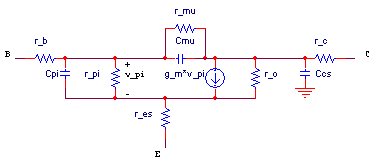
\includegraphics{schematics/complete_bipolar_hybrid_pi.PNG}
	\caption{Complete bipolar hybrid-pi model}
	\label{fig:complete_bipolar_hybrid_pi}
\end{figure}
\begin{figure}[h]
	\centering
		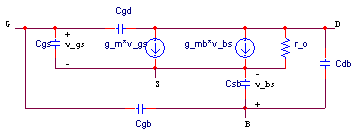
\includegraphics{schematics/complete_MOS_ss_model.PNG}
	\caption{Complete MOS small-signal model}
	\label{fig:complete_MOS_ss_model}
\end{figure}

It is usually not necessary to use the complete hybrid-$\pi$ or MOS small signal model, and attempting to use the complete models usually makes the small-signal analysis overly complicated.
For hand calculations with the hybrid-$\pi$ small-signal model one can usually treat $C_{\pi}$, $r_{\mu}$, $C_{\mu}$, and $C_{cs}$ as open circuits, and $r_{es}$ and $r_{c}$ as a short circuit.
For hand calculations with the MOS small-signal model one can usually treat all the capacitors as open circuits.
Additionally, one can usually ignore the $g_{mb}v_{bs}$ dependent current source since the MOSFET's backgate is usually connected to the source.
Unless specifically stated otherwise, the following analyses assume the backgate is connected to the source so $g_{mb}v_{bs} = 0$.

\section{Common emitter/source}
\begin{center}
	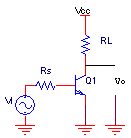
\includegraphics{schematics/basiccommonemitter.PNG}
\end{center}
\par
The common emitter (or common source) is so named because in this configuration the emitter/source of the transistor is shorted to a common signal source (in this case, $GND$). The output is taken from the transistor's collector (or drain). Sometimes the common emitter/source is used with a resistor connected from the emitter/source to the common signal source; such a resistor is called an \textit{emitter degeneration} resistor or \textit{source degeneration} resistor. Emitter/source degeneration employs negative feedback in the form of an impedance to provide temperature stability to the circuit at DC -- a common emitter without emitter degeneration has $v_{BE} = v_{B} = v_{I}$ (where $v_{B}$ is the voltage at the transistor's base) and $i_{C} = I_{S}e^{\frac{v_{I}}{V_{th}}}$ so $v_{O} = V_{CC} - R_{L}I_{S}e^{\frac{v_{I}}{V_{th}}}$. Lack of emitter degeneration therefore gives high gain (since the $v_{I}$ term is part of an exponential) at the expense of temperature stability (since the temperature-dependent $V_{th}$ term is also in the exponential). Such a tradeoff is a familiar concept in control theory. For an AC signal, however, emitter/source degeneration can be used to provide DC stability without sacrificing gain by using an appropriately sized emitter/source capacitor $C_{E}$ (or $C_{S}$) in parallel with the emitter/source degeneration resistor $R_{E}$ (or $R_{S}$) that has (ideally) zero impedance at all frequencies of the input signal. The DC stability provided by the emitter degeneration resistor ensures that the transistor is biased correctly so that it behaves linearly for the small signal input while the emitter/source capacitor maintains high gain for input AC signals.
\par
If the common emitter/source is used for processing AC signals but not DC, it is usually necessary to use a DC blocking capacitor in series with the output of the preceding stage and the transistor's base. Figure \ref{fig:commonemitter} shows the common emitter with a DC blocking capacitor, a voltage divider to bias the transistor's base, an emitter degeneration resistor, and an emitter bypass capacitor.

\subsection{Bipolar}
\begin{figure}[h]
	\centering
		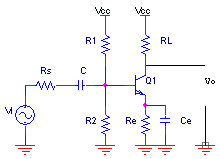
\includegraphics{schematics/commonemitter.PNG}
	\caption{Common emitter implementation for AC signals}
	\label{fig:commonemitter}
\end{figure}
\par
To analyze the small signal behavior of the common emitter one can use a slightly simplified version of the hybrid-$\pi$ small signal model. Also, assume the DC blocking capacitor is a short circuit for the frequencies of interest and, to derive as general a transfer function as possible, assume an emitter degeneration resistor is used without an emitter bypass capacitor. For simplicity assume that $R_{1}$ and $R_{2}$ are large enough that they can be ignored and define $R_{S}' = R_{S}+r_{b}$. Figure \ref{fig:ss_commonemitter} shows the small signal model of this common emitter circuit.
\begin{figure}[h]
	\centering
		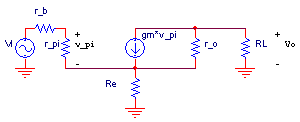
\includegraphics{schematics/ss_commonemitter.PNG}
	\caption{Common emitter small signal model}
	\label{fig:ss_commonemitter}
\end{figure}
\par
It is easy enough to derive the transfer function of the common emitter without emitter degeneration since with $R_{E} = 0$ the emitter is shorted to ground and the input section ($v_{i}$, $r_{b}$, and $r_{\pi}$) is isolated from the output section ($g_{m}v_{\pi}$, $r_{o}$, and $R_{L}$). However, for the general case (i.e. with emitter degeneration) it is easier to view the common emitter as an equivalent two port small-signal model as shown in Figure \ref{fig:twoport_ss_model} and derive the input resistance $R_{i}$, output resistance $R_{o}$, and transconductance $G_{m}$ (note that $G_{m}$ is not to be confused with the transistor's transconductance $g_{m}$ -- it is $G_{m} = \frac{i_{o}}{v_{i}}$ with the output shorted).
\begin{figure}
	\centering
		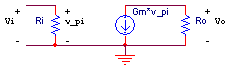
\includegraphics{schematics/twoport_ss_model.PNG}
	\caption{Two port equivalent small-signal model}
	\label{fig:twoport_ss_model}
\end{figure}
\par
To derive $R_{i}$, $R_{o}$, and $G_{m}$ start with Ohm's Law and KCL at the emitter and collector. By Ohm's Law,

\begin{equation}
i_{b} = \frac{v_{i}-v_{e}}{r_{\pi}}
\label{eq:common_emitter_i_b}
\end{equation}

\noindent (where $v_{e}$ is the voltage at the emitter and $i_{b}$ is the small-signal base current and also the circuit's small-signal input current). KCL at the emitter yields

\begin{equation}
\frac{v_{e}}{R_{E}} + \frac{v_{e}+i_{o}R_{L}}{r_{o}} = (\beta_{0}+1)i_{b}
\label{eq:common_emitter_KCL_emitter}
\end{equation}

\noindent (recall that $g_{m}v_{\pi} = \beta_{0}i_{b}$). KCL at the collector yields

\begin{equation}
i_{o} + \frac{v_{e}+i_{o}R_{L}}{r_{o}} = i_{o}\left(1 + \frac{R_{L}}{r_{o}}\right) + \frac{v_{e}}{r_{o}} = \beta_{0}i_{b}
\label{eq:common_emitter_KCL_collector}
\end{equation}

\noindent Solving for $i_{o}$ in (\ref{eq:common_emitter_KCL_emitter}), substituting it into (\ref{eq:common_emitter_KCL_collector}), and rearranging, we find

\begin{equation}
v_{e} = i_{b}\left(\frac{1+(\beta_{0}+1)\frac{r_{o}}{R_{L}}}{\frac{1}{R_{L}} + \frac{1}{R_{E}} + \frac{r_{o}}{R_{L}R_{E}}}\right)
\label{eq:common_emitter_v_e}
\end{equation}

Substituting (\ref{eq:common_emitter_v_e}) into (\ref{eq:common_emitter_i_b}) (which can be rewritten as $R_{i} = \vin/i_b = \rpi + v_e/i_b$), we find \autocite[197-199]{analysis-design-analog-ics}

\textcolor{red}{
\begin{equation}
R_{i} = r_{\pi} + (\beta_{0}+1)\left(\frac{r_{o} + \frac{R_{L}}{\beta_{0}+1}}{r_{o} + R_{L} + R_{E}}\right)R_{E}
\label{eq:common_emitter_Ri}
\end{equation}
}

\par
Often $r_{o} >> R_{L}$ and $r_{o} >> R_{E}$ so (\ref{eq:common_emitter_Ri}) can be approximated as

\textcolor{red}{
\begin{equation}
R_{i} \approx r_{\pi} + (\beta_{0}+1)R_{E}
\label{eq:common_emitter_Ri_approx}
\end{equation}
}

Note that this approximation is consistent with the principle of \textit{$\beta_{F}$ impedance reflection}.

For the circuit's transconductance $G_{m}$ set $R_{L} = 0$ (since the output is shorted by definition of $G_{m}$). From the emitter KCL equation $\frac{v_{e}}{R_{E}} + \frac{v_{e}}{r_{o}} = (\beta_{0} + 1)i_{b} = (\beta_{0} + 1)\frac{v_{i}-v_{e}}{r_{\pi}}$ so

\begin{equation}
v_{e} = \frac{\frac{\beta_{0}+1}{r_{\pi}}}{\frac{1}{R_{E}} + \frac{1}{r_{o}} + \frac{1}{r_{\pi}}}v_{i}
\label{eq:common_emitter_v_e2}
\end{equation}

From the collector KCL equation we know

\begin{equation}
i_{o} + \frac{v_{e}}{r_{o}} = \beta_{0}i_{b} = \beta_{0}\frac{v_{i}-v_{e}}{r_{\pi}}
\label{eq:common_emitter_KCL_collector2}
\end{equation}

so we can substitute (\ref{eq:common_emitter_v_e2}), which is in terms of \vin, to find \autocite[199]{analysis-design-analog-ics}

\textcolor{red}{
\begin{equation}
G_{m} = g_{m}\frac{1-\frac{R_{E}}{\beta_{0}r_{o}}}{1 + g_{m}R_{E}\left(1 + \frac{1}{\beta_{0}} + \frac{1}{g_{m}r_{o}}\right)}
\label{eq:common_emitter_Gm}
\end{equation}
}

Often $r_{o} \gg R_{E}$, $\beta_{0} \gg 1$, and $g_{m}r_{o} \gg 1$ so

\textcolor{red}{
\begin{equation}
G_{m} \approx \frac{g_{m}}{1 + g_{m}R_{E}}
\label{eq:common_emitter_Gm_approx}
\end{equation}
}

Without emitter degeneration ($R_{E} = 0$) both equations reduce to $G_{m} = g_{m}$, which is expected since the common emitter's hybrid-$\pi$ small-signal model looks like the two port small-signal model when the emitter is shorted to ground.

It is clear from the two port model (Figure \ref{fig:twoport_ss_model}) that $\vout = -G_{m}r_{o}\vin$ so using (\ref{eq:common_emitter_Gm}) we know

\textcolor{red}{
\begin{equation}
\frac{\vout}{\vin} = g_{m}\frac{1-\frac{R_E}{\beta_0 r_o}}{1 + g_m R_E\left(1 + \frac{1}{\beta_0} + \frac{1}{g_m r_o}\right)}r_o
\label{eq:commonemitter_transferfunction}
\end{equation}
}

\begin{figure}
	\centering
		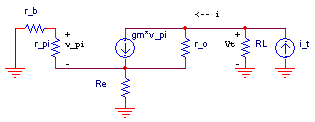
\includegraphics{schematics/commonemitter_Ro.PNG}
	\caption{Common emitter small-signal equivalent model for computing output resistance}
	\label{fig:commonemitter_Ro}
\end{figure}

To find the small-signal output resistance $R_{o}$ of the common emitter, use the equivalent circuit shown in Figure \ref{fig:commonemitter_Ro}. Using a test current source $i_{t}$ and the voltage $v_{t}$ across it, $R_{o}$ is, by definition,

\begin{equation}
R_{o} = \frac{v_{t}}{i_{t}}
\end{equation}

\noindent By defining $i$ as the portion of the $i_{t}$ current into the $g_{m}v_{\pi}$ current source and $r_{o}$, this becomes

\begin{equation}
R_{o} = \frac{v_{t}}{i}||R_{L}
\end{equation}

\noindent The current $i$ splits between the $g_{m}v_{\pi}$ current source and $r_{o}$ but recombines at the emitter node so

\begin{equation}
v_{\pi} = -i\frac{r_{\pi}R_{E}}{r_{\pi}+R_{E}}
\label{eq:commonemitter_Ro_v_pi}
\end{equation}

\noindent assuming $r_{b}$ is small enough to be ignored (if not, simply add it to $r_{\pi}$). Also, the current $i_{1}$ through $r_{o}$ is

\begin{equation}
i_{1} = i - g_{m}v_{\pi} = i + ig_{m}\frac{r_{\pi}R_{E}}{r_{\pi}+R_{E}}
\label{eq:commonemitter_Ro_i_1}
\end{equation}

\noindent where the latter equation is true by substituting $-i(r_{\pi}||R_{E})$ for $v_{\pi}$ using (\ref{eq:commonemitter_Ro_v_pi}). Using (\ref{eq:commonemitter_Ro_v_pi}) and (\ref{eq:commonemitter_Ro_i_1}), the voltage $v_{t}$ is thus

\begin{equation}
v_{t} = i_{1}r_{o}-v_{\pi} = i\frac{r_{\pi}R_{E}}{r_{\pi}+R_{E}} + ir_{o}\left(1+g_{m}\frac{r_{\pi}R_{E}}{r_{\pi}+R_{E}}\right)
\label{eq:commonemitter_Ro_v_t}
\end{equation}

\noindent Dividing both sides of (\ref{eq:commonemitter_Ro_v_t}) by $i$ and putting the result in parallel with $R_{L}$ gives \autocite[200]{analysis-design-analog-ics}

\textcolor{red}{
\begin{equation}
R_{o} = \left(\frac{r_{\pi}R_{E}}{r_{\pi}+R_{E}} + r_{o}\left(1+g_{m}\frac{r_{\pi}R_{E}}{r_{\pi}+R_{E}}\right)\right) \parallel R_{L}
\label{eq:commonemitter_Ro}
\end{equation}
}

The first term is much smaller than the second so
\textcolor{red}{
\begin{equation}
R_{o} \approx r_{o}\left(1+g_{m}\frac{r_{\pi}R_{E}}{r_{\pi}+R_{E}}\right) \parallel R_{L} = r_{o}\left(1+\frac{g_{m}R_{E}}{1+\frac{g_{m}R_{E}}{\beta_{0}}}\right) \parallel R_{L}
\end{equation}
}

Depending on whether $\beta_{0}$ is significantly larger or smaller than $g_{m}R_{E}$, $R_{o}$ can be further simplified as follows:

\textcolor{red}{
\begin{equation}
R_{o} \approx (r_{o}(1+g_{m}R_{E})) \parallel R_{L}\text{, }\beta_{0} \gg g_{m}R_{E}
\end{equation}
}

\textcolor{red}{
\begin{equation}
R_{o} \approx (r_{o}(1+\beta_{0})) \parallel R_{L}\text{, }g_{m}R_{E} \gg \beta_{0}
\end{equation}
}

\subsection{MOS}
The small signal model of the common source is identical to the common emitter hybrid-$\pi$ model shown in Figure \ref{fig:ss_commonemitter}, except that $r_{\pi} \rightarrow \infty$ and the $g_{m}v_{\pi}$ current source is replaced with two current sources ($g_{m}v_{gs}$ and $g_{mb}v_{bs}$) in parallel (assuming the body terminal is connected to GND or $V_{SS}$, whichever is the lowest supply voltage). First we find $G_{m} = \frac{i_{o}}{v_{i}}$ using KCL at the source and at the drain (with $R_{L} = 0$):

\begin{equation}
\frac{v_{s}}{R_{S}} + \frac{v_{s}}{r_{o}} = g_{m}v_{gs} + g_{mb}v_{bs} = g_{m}(v_{i}-v_{s}) - g_{mb}v_{s}
\label{eq:commonsource_KCL_source}
\end{equation}

\begin{equation}
i_{o} + \frac{v_{s}}{r_{o}} = g_{m}v_{gs} + g_{mb}v_{bs} = g_{m}(v_{i}-v_{s}) - g_{mb}v_{s}
\label{eq:commonsource_KCL_drain}
\end{equation}

Solving (\ref{eq:commonsource_KCL_source}) for $v_{s}$ yields

\begin{equation}
v_{s} = \frac{g_{m}v_{i}}{g_{m}+g_{mb}+\frac{1}{R_{S}}+\frac{1}{r_{o}}}
\label{eq:commonsource_v_s}
\end{equation}

Substituting (\ref{eq:commonsource_v_s}) into (\ref{eq:commonsource_KCL_drain}) and rearranging yields \autocite[201]{analysis-design-analog-ics}

\textcolor{red}{
\begin{equation}
G_{m} = \frac{g_{m}}{1+(g_{m}+g_{mb})R_{S}+\frac{R_{S}}{r_{o}}}
\end{equation}
}

In the case where $r_{o} \gg R_{S}$, the equation for $G_{m}$ simplifies to

\textcolor{red}{
\begin{equation}
G_{m} \approx \frac{g_m}{1+(g_m + g_{mb})R_S}
\end{equation}
}

The common source's output resistance $R_{o}$ can be computed the same way as the common emitter's $R_{o}$: we apply a test current $i_{t}$ into the output and measure the voltage $v_{t}$ across the current source (as before, temporarily ignore $R_{L}$ and add it back in parallel) to find $R_{o} = \frac{v_{t}}{i_{t}}$.
The test current $i_{t}$ is also the current through $R_{S}$ since none of it is diverted through a finite $r_{\pi}$ so

\begin{equation}
v_{s} = i_{t}R_{S}
\label{eq:commonsource_Ro_v_s}
\end{equation}

If $i_{1}$ is the current through $r_{o}$, \ac{kvl} shows that

\begin{equation}
v_{t} = i_{1}r_{o}+v_{s} = (i_{t}-g_{m}v_{gs}-g_{mb}v_{bs})r_{o}+v_{s} = (i_{t}+g_{m}v_{s}+g_{mb}v_{s})r_{o}+v_{s}
\label{eq:commonsource_Ro_v_t}
\end{equation}

\noindent Substituting (\ref{eq:commonsource_Ro_v_s}) into (\ref{eq:commonsource_Ro_v_t}), rearranging, and then putting the result in parallel with $R_{L}$ yields

\textcolor{red}{
\begin{equation}
R_{o} = (R_{S} + (1+(g_{m}+g_{mb})R_{S})r_{o}+R_{S}) \parallel R_{L}
\label{eq:commonsource_Ro}
\end{equation}
}

The common source's input resistance $R_{i}$ is trivially

\textcolor{red}{
\begin{equation}
R_{i} = \infty
\end{equation}
}

\section{Common collector/drain (emitter/source follower)}
\begin{center}
	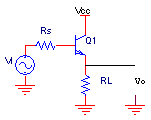
\includegraphics{schematics/basicemitterfollower.PNG}
\end{center}

In this circuit the collector or drain is shorted to the supply voltage so it is called a common collector (or common drain). It is also known as the emitter follower (or source follower) since \vout is the voltage across the emitter (or source) resistor and follows the base voltage (which is also the input voltage \vin). The circuit has a voltage gain of approximately unity so it is a voltage follower (buffer).

As will be seen in the full analysis, emitter/source followers have a high $R_{i}$. This makes them useful loads for voltage amplifiers (such as common emitters/sources) so that most of the preceding amplifier's output voltage falls across the emitter/source follower's input. The full analysis will also show that emitter/source followers have a low $R_{o}$, which makes them useful sources for circuits that require an input voltage since an ideal voltage source has zero $R_{o}$. Emitter/source followers are also used to push out poles that would otherwise appear in a circuit by reducing the resistance seen by a node where a capacitance appears (a high resistance seen by a capacitor can result in a long RC time constant, degrading the circuit's response at higher frequencies). Emitter/source followers are thus highly useful circuits even when processing voltage signals.

\subsection{Bipolar}
For the emitter follower it is easy to see from (\ref{eq:bipolarIc}) that the voltage gain is approximately unity even without a full analysis. Assuming a constant temperature so $V_{TH}$ does not vary, $v_{BE}$ does not vary significantly even for relatively large variations in $I_{C}$ due to the exponential relationship between $v_{BE}$ and $I_{C}$. Since $v_{BE}$ does not vary then $v_{E} = v_{O}$ must follow $v_{B} = v_{I}$.
\begin{figure}[h]
	\centering
		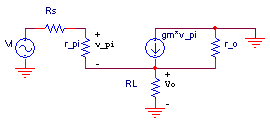
\includegraphics{schematics/ss_emitterfollower.PNG}
	\caption{Emitter follower small signal model}
	\label{fig:ss_emitterfollower}
\end{figure}

Although the preceding first order analysis proves that the voltage gain is approximately unity, it is often necessary to know the exact transfer function. To find it, use KCL at the emitter:

\begin{equation}
i_{i}+\beta_{0} i_{i} - \frac{v_{o}}{R_{L}} - \frac{v_{o}}{r_{o}} = 0
\label{eq:emitter_follower_KCL_output}
\end{equation}

\noindent where $i_{i}$ is the current into the base of the transistor. Since $i_{i}$ flows through $R_{S}$ (which may include the transistor's base resistance $r_{b}$, if such accuracy is needed) and $r_{\pi}$, and the voltage across these two resistors is $v_{be} = v_{i} - v_{o}$, 

\begin{equation}
i_{i} = \frac{v_{i}-v_{o}}{R_{S}+r_{\pi}}
\label{eq:emitter_follower_i_i}
\end{equation}

\noindent Substituting into (\ref{eq:emitter_follower_KCL_output}) and rearranging terms, the transfer function is

\textcolor{red}{
\begin{equation}
\frac{v_{o}}{v_{i}} = \frac{1}{1+\frac{R_{S}+r_{\pi}}{(\beta_{0} + 1)(R_{L}||r_{o})}}
\label{eq:emitter_follower}
\end{equation}
}

\noindent If $(\beta_{0} + 1)(R_{L}||r_{o}) >> R_{S}+r_{\pi}$ then the voltage gain is approximately unity. Another common approximation of the transfer function is

\textcolor{red}{
\begin{equation}
\frac{v_{o}}{v_{i}} \approx \frac{g_{m}R_{L}}{1+g_{m}R_{L}}
\label{eq:emitter_follower_approx}
\end{equation}
}

\noindent which is true when $\beta >> 1$, $r_{\pi} >> R_{S}$, and $r_{o} >> R_{L}$.
\par
The input resistance $R_{i}$ of the emitter follower can be determined by removing the input voltage source (including its resistance $R_{S}$) and measuring the equivalent resistance looking into the input terminals. Similarly, the output resistance $R_{o}$ can be determined by removing the load resistor $R_{L}$ and measuring the equivalent resistance looking into the output terminals. However, both $R_{i}$ and $R_{o}$ can be determined by inspection using \textit{impedance reflection}:

\textcolor{red}{
\begin{equation}
R_{i} = r_{\pi} + (\beta_{0} + 1)(R_{L}||r_{o})
\label{eq:emitter_follower_Ri}
\end{equation}
}

\textcolor{red}{
\begin{equation}
R_{o} = \frac{R_{S}+r_{\pi}}{\beta_{0} + 1}||r_{o}
\label{eq:emitter_follower_Ro}
\end{equation}
}

\noindent The latter simplifies to

\textcolor{red}{
\begin{equation}
R_{o} \approx \frac{1}{g_{m}} + \frac{R_{S}}{\beta_{0} + 1}
\label{eq:emitter_follower_Ro_approx}
\end{equation}
}

\noindent if $\beta >> 1$ and $r_{o} >> \frac{R_{S}+r_{\pi}}{\beta_{0} + 1}$.
\newpage
\begin{figure}[h]
	\centering
		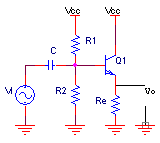
\includegraphics{schematics/emitterfollower.PNG}
	\caption{Emitter follower implementation for AC signals}
	\label{fig:emitterfollowerAC}
\end{figure}
\par
An emitter follower implementation for AC signals is shown above in Figure \ref{fig:emitterfollowerAC}. It includes bias resistors $R_{1}$ and $R_{2}$ which of course affect $R_{i}$ -- add $R_{1}||R_{2}$ in parallel with (\ref{eq:emitter_follower_Ri}).

\subsection{MOS}
The source follower also has a voltage gain of approximately unity, a fact which can be seen from the square-law dependence of $I_{D}$ on $V_{GS}$ in the active region as shown by (\ref{eq:activeId}) -- $V_{GS}$ does not vary significantly even for relatively large variations in $I_{D}$. $V_{GS}$ does vary with $I_{D}$ more than the bipolar transistor's $V_{BE}$ varies with its $I_{C}$, however, so a source follower's voltage gain is generally less than unity and more so than the emitter follower's voltage gain. The full small signal analysis will demonstrate this.
\begin{figure}[h]
	\centering
		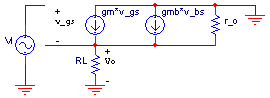
\includegraphics{schematics/ss_sourcefollower.PNG}
	\caption{Source follower small signal model}
	\label{fig:ss_sourcefollower}
\end{figure}
\par
With the MOSFET's body terminal connected to the lowest supply voltage (GND) in the small signal model shown in Figure \ref{fig:ss_sourcefollower}, we can determine the transfer function exactly by realizing that

\begin{equation}
v_{bs} = -v_{s} = -v_{o}
\end{equation}

\noindent and finding KCL at the output (the source):

\begin{equation}
g_{m}v_{gs} - g_{mb}v_{o} = \frac{v_{o}}{R_{L}} + \frac{v_{o}}{r_{o}}
\label{eq:sourcefollower_KCL}
\end{equation}

\noindent Also, KVL around the input loop shows that

\begin{equation}
v_{i} = v_{o} + v_{gs}
\label{eq:sourcefollower_KVL}
\end{equation}

\noindent Solving (\ref{eq:sourcefollower_KCL}) for $v_{gs}$ and substituting the result into (\ref{eq:sourcefollower_KVL}) gives

\textcolor{red}{
\begin{equation}
\frac{v_{o}}{v_{i}} = \frac{g_{m}}{g_{m} + g_{mb} + \frac{1}{R_{L}} + \frac{1}{r_{o}}} = \frac{g_{m}r_{o}}{(g_{m} + g_{mb})r_{o} + 1 + \frac{r_{o}}{R_{L}}}
\label{eq:sourcefollower}
\end{equation}
}

\noindent In the case where $R_{L} \rightarrow \infty$, (\ref{eq:sourcefollower}) simplifies to

\textcolor{red}{
\begin{equation}
\frac{v_{o}}{v_{i}} \approx \frac{g_{m}r_{o}}{1+(g_{m}+g_{mb})r_{o}}
\end{equation}
}

% TODO: figure out how to do lim -> \infty
\noindent If both $R_{L} \rightarrow \infty$ and $r_{o} \rightarrow \infty$ then

\begin{equation}
\frac{v_{o}}{v_{i}} \approx \frac{g_{m}}{g_{m}+g_{mb}} = \frac{1}{1+\chi}
\end{equation}

\noindent where $\chi$ is defined in (\ref{eq:chi}) and is typically well below unity (in the range of 0.2).
\par
The voltage gain can be improved by tying the MOSFET's body to its source so that $v_{bs} = 0$ and the $g_{mb}$ term disappears:

\textcolor{red}{
\begin{equation}
\frac{v_{o}}{v_{i}} = \frac{g_{m}r_{o}}{1+g_{m}r_{o} + \frac{r_{o}}{R_{L}}}
\label{eq:sourcefollower_no_gmb}
\end{equation}
}

\textcolor{red}{
\begin{equation}
\frac{v_{o}}{v_{i}} \approx \frac{g_{m}r_{o}}{1+g_{m}r_{o}}
\end{equation}
}

The input resistance $R_{i}$ of the source follower is the resistance looking into the gate of the MOSFET, which is trivially

\textcolor{red}{
\begin{equation}
R_{i} = \infty
\end{equation}
}

The output resistance $R_{o}$ is the resistance looking into the output with $v_{i} = 0$. Since $v_{i} = 0$ it is obvious that

\begin{equation}
v_{gs} = -v_{o}
\end{equation}

\noindent Also, KCL at the output yields

\begin{equation}
i_{o} = \frac{v_{o}}{r_{o}} + \frac{v_{o}}{R_{L}} + (g_{m}+g_{mb})v_{o}
\label{eq:sourcefollower_Ro_io}
\end{equation}

\noindent Rearranging (\ref{eq:sourcefollower_Ro_io}) gives an equation for $R_{o}$:

\textcolor{red}{
\begin{equation}
R_{o} = \frac{1}{g_{m}+g_{mb}+\frac{1}{r_{o}}+\frac{1}{R_{L}}}
\label{eq:sourcefollower_Ro}
\end{equation}
}

\section{Common base/gate}
\begin{center}
	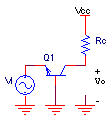
\includegraphics{schematics/commonbase.PNG}
\end{center}
The transistor in a common base/gate circuit is biased such that the base/gate is directly connected to AC ground, the input is applied to the emitter/source, and the output is taken from the collector/drain. Although the input and output signals are voltages, it is useful to think of the common base/gate as a current source (since $I_{C} \approx I_{E}$ and $I_{D} \approx I_{S}$) with a high $R_{o}$ (the resistance looking into the collector/drain is $r_{o}$, which is usually very high). These characteristics of the common base/gate make it useful in certain situation, such as a cascode circuit (see below).

\subsection{Bipolar}
\par
The transfer function and input and output resistances of the previous circuits were derived using the hybrid-$\pi$ small signal model, but the dependent $g_{m}v_{\pi}$ current source is directly connected from output to input and thus makes the analysis of the hybrid-$\pi$ small signal model for the common base difficult. One way to simplify the analysis of the common base circuit is to transform the hybrid-$\pi$ model into an equivalent \textsl{T model}. The first step in this tranformation is to split the $g_{m}v_{\pi}$ current source into two current sources of value $g_{m}v_{\pi}$, with one connected from the collector to the base and the other connected from the base to the emitter. Splitting the $g_{m}v_{\pi}$ current source like this is possible since the currents entering and exiting the base are equal (i.e. KCL at the base is unchanged) and the two current sources supply the same current from collector to emitter. Next, note that the $g_{m}v_{\pi}$ dependent current source from the collector to the base is controlled by the voltage across it -- so its equivalent resistance $r_{cb}$ is

\begin{equation}
r_{cb} = \frac{v_{\pi}}{g_{m}v_{\pi}} = \frac{1}{g_{m}}
\end{equation}

\noindent and we can replace the dependent current source with a resistor that is in parallel with $r_{\pi}$. The parallel combination of these two resistors is the equivalent resistance $r_{e}$, which is

\begin{equation}
r_{e} = \frac{\frac{r_{\pi}}{g_{m}}}{\frac{1}{g_{m}}+r_{\pi}} = \frac{1}{\frac{1}{r_{\pi}}+g_{m}} = \frac{1}{g_{m}\left(1+\frac{1}{\beta_{0}}\right)}
\end{equation}

At low frequencies the capacitors and resistors $r_{o}$ and $r_{\mu}$ can be neglected, in which case the small signal model looks like a ``T''. The transformation from the hybrid-$\pi$ model to the \textsl{T model} with and without the higher frequency elements is shown in Figures \ref{fig:ss_commonbase_hybrid_pi} - \ref{fig:ss_commonbase_T_model_approx}. \autocite[183-184]{analysis-design-analog-ics}

\begin{figure}[h]
	\centering
		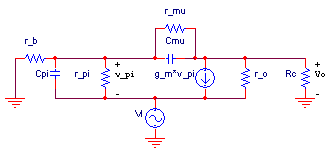
\includegraphics{schematics/ss_commonbase_hybrid_pi.PNG}
	\caption{Hybrid-$\pi$ small signal model for common base analysis}
	\label{fig:ss_commonbase_hybrid_pi}
\end{figure}

\begin{figure}[h]
	\centering
		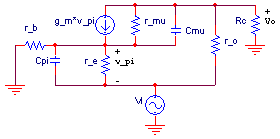
\includegraphics{schematics/ss_commonbase_T_model.PNG}
	\caption{Small signal \textsl{T model} for common base analysis}
	\label{fig:ss_commonbase_T_model}
\end{figure}

\begin{figure}[h]
	\centering
		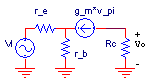
\includegraphics{schematics/ss_commonbase_T_model_approx.PNG}
	\caption{Small signal \textsl{T model} for common base at low frequencies}
	\label{fig:ss_commonbase_T_model_approx}
\end{figure}

With this simplified model it is trivial to see that

\textcolor{red}{
\begin{equation}
R_{o} = R_{C}
\label{eq:common_base_Ro}
\end{equation}
}

It is also easy to see that the short-circuit transconductance is

\begin{equation}
G_{m} = \frac{i_{o}}{v_{i}}|_{v_{o}=0} = \frac{g_{m}v_{\pi}}{v_{i}}
\label{eq:commonbase_Gm_initial}
\end{equation}

since $v_{\pi}$ is the voltage across $r_{e}$. We need to know the relationship between $v_{\pi}$ and $v_{i}$, however, in order to derive a useful expression for $G_{m}$ and $R_{i}$. This relationship can be found by KVL around the input loop

\begin{equation}
v_{i} = v_{b} + v_{e}
\end{equation}

and \ac{kcl} at the node between $r_{e}$ and $r_{b}$ (the transistor's base):

\begin{equation}
g_{m}v_{\pi} + \frac{v_{b}}{r_{b}} = \frac{v_{e}}{r_{e}}
\label{eq:commonbase_KCL_base}
\end{equation}

Substituting for $v_{b}$ in (\ref{eq:commonbase_KCL_base}) we find that

\begin{equation}
\frac{v_{i}}{v_{\pi}} = 1 + \frac{g_{m}}{\beta_{0}}r_{b} = 1 + \frac{r_{b}}{r_{\pi}}
\label{eq:commonbase_vi_vpi}
\end{equation}

Now a simple substitution from (\ref{eq:commonbase_vi_vpi}) into (\ref{eq:commonbase_Gm_initial}) gives \autocite[185]{analysis-design-analog-ics}

\textcolor{red}{
\begin{equation}
G_{m} = \frac{g_{m}}{1+\frac{r_{b}}{r_{\pi}}}
\end{equation}
}

Since the relationship between $v_{i}$ and $v_{\pi}$ is known and

\begin{equation}
R_{i} = \frac{v_{i}}{i_{i}} = \frac{v_{i}}{v_{\pi}}r_{e}
\end{equation}

by inspection, we know

\textcolor{red}{
\begin{equation}
R_{i} = r_{e}\left(1 + \frac{r_{b}}{r_{\pi}}\right)
\end{equation}
}

We can now calculate the voltage and current gain of the common base:

\textcolor{red}{
\begin{equation}
\frac{\vout}{\vin} = G_{m}R_{o} = \frac{g_{m}R_{C}}{1+\frac{r_{b}}{r_{\pi}}}
\end{equation}
}

\textcolor{red}{
\begin{equation}
\frac{i_{o}}{i_{i}} = G_{m}R_{i} = g_{m}r_{e}
\end{equation}
}

\subsection{MOS}
As with the common base, the analysis of the common gate may be simplified by transforming the transistor's small signal model into an equivalent \textsl{T model}.
From the small signal model, the $g_{m}v_{gs}$ and $g_{mb}v_{bs}$ current sources can be combined if the MOSFET body is connected to ground (which we will assume).
The combined current source $(g_{m}+g_{mb})v_{gs}$ can then be split into two current sources of equal magnitude and opposite direction to ground since \ac{kcl} at the source and drain are unaffected and no net current enters or leaves ground.
Next, the current source $(g_{m}+g_{mb})v_{gs}$ between the gate and source is controlled by the voltage across it so it is equivalently a resistor of value $1/(g_{m}+g_{mb})$.
Figures \ref{fig:ss_commongate_initial} - \ref{fig:ss_commongate_T_model} show this transformation. \autocite[186]{analysis-design-analog-ics}

\begin{figure}[h]
	\centering
		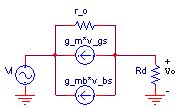
\includegraphics{schematics/ss_commongate_initial.PNG}
	\caption{Small signal model for the common gate circuit}
	\label{fig:ss_commongate_initial}
\end{figure}

\begin{figure}[h]
	\centering
		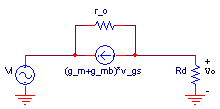
\includegraphics{schematics/ss_commongate_combine.PNG}
	\caption{Common gate small signal model with current sources combined}
	\label{fig:ss_commongate_combine}
\end{figure}

\begin{figure}[h]
	\centering
		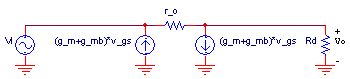
\includegraphics{schematics/ss_commongate_split.PNG}
	\caption{Common gate small signal model with current source split}
	\label{fig:ss_commongate_split}
\end{figure}

\begin{figure}[h]
	\centering
		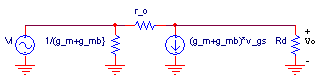
\includegraphics{schematics/ss_commongate_T_model.PNG}
		\caption{Common gate \textsl{T model}}
	\label{fig:ss_commongate_T_model}
\end{figure}

Assuming $r_{o} \to \infty$ we can determine the circuit's parameters by inspection:

\begin{equation}
G_{m} = g_{m} + g_{mb}
\end{equation}

\textcolor{red}{
\begin{equation}
R_{i} = \frac{1}{g_{m}+g_{mb}}
\end{equation}
}

\textcolor{red}{
\begin{equation}
R_{o} = R_{D}
\label{eq:common_gate_Ro}
\end{equation}
}

\textcolor{red}{
\begin{equation}
\frac{v_{o}}{v_{i}} = G_{m}R_{o} = (g_{m}+g_{mb})R_{D}
\end{equation}
}

\textcolor{red}{
\begin{equation}
\frac{i_{o}}{i_{i}} = G_{m}R_{i} = 1
\end{equation}
}

\section{Cascode}
\begin{center}
	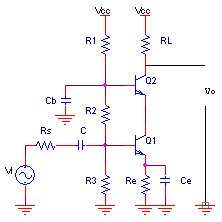
\includegraphics{schematics/cascode.PNG}
\end{center}
The cascode is a two transistor circuit that is actually a first stage common emitter/source driving a second stage common base/gate. To analyze the small signal voltage gain, we will approximate

\begin{equation}
i_{c1} = i_{e2} = \left(1+\frac{1}{\beta}\right)i_{c2}
\end{equation}

\noindent as

\begin{equation}
i_{c1} \approx i_{c2}
\end{equation}

\noindent This approximation is valid if $\beta_{0} >> 1$. Under this approximation 

\begin{equation}
g_{m1} = g_{m2}
\end{equation}

\noindent and

\begin{equation}
r_{\pi 1} = r_{\pi 2}
\end{equation}

\noindent We define these as $g_{m}$ and $r_{\pi}$, respectively. From the circuit configuration

\begin{equation}
v_{o} = -i_{c2}(R_{L}||r_{o}) \approx -i_{c1}(R_{L}||r_{o})
\end{equation}

\noindent and from the small signal model

\begin{equation}
i_{c1} = g_{m}v_{\pi 1} = g_{m}\frac{r_{\pi}}{r_{\pi}+ R'_{S}}v_{i}
\end{equation}

\noindent Substituting gives

\begin{equation}
v_{o} = -g_{m}\frac{r_{\pi}}{r_{\pi}+ R'_{S}}(R_{L}||r_{o})v_{i}
\end{equation}

\noindent Rearranging and noting that $\beta_{0} = g_{m}r_{\pi}$ we find

\textcolor{red}{
\begin{equation}
\frac{v_{o}}{v_{i}} = -\frac{\beta_{0} (R_{L}||r_{o})}{r_{\pi}+ R'_{S}}
\end{equation}
}

\par
This is the same voltage gain as the common emitter! Compared to the common emitter the cascode requires an extra transistor and additional bias circuitry, suffers from reduced signal swing (since $v_{o}$ is limited by two $v_{BE}$ drops rather than one), and offers the same voltage gain. Why would one ever use a cascode rather than just a common emitter? The key improvement of the cascode over the common emitter is its bandwidth. The resistance seen by $Q_{1}$'s $C_{\mu}$ for both the cascode and common emitter is

\begin{equation}
R'_{S}||r_{\pi} + (1 + g_{m}(R'_{S}||r_{\pi}))R_{LOAD}
\end{equation}

where $R_{LOAD}$ is the load resistance on the common emitter stage. By definition $R_{LOAD} = R_{L}$ for the common emitter, but $R_{LOAD} \approx \frac{1}{g_{m}}$ for the cascode ($C_{B}$ shorts $Q_{2}$'s base to AC ground so that the bias resistors do not affect $R_{LOAD}$). $R_{L}$ is usually much higher than $\frac{1}{g_{m}}$ (and it must be in order to acheive a high voltage gain) so this open circuit time constant is much smaller for the cascode than the common emitter, yet the cascode offers the same gain as the common emitter. The cascode is thus an extremely useful circuit for high gain while maintaining a high bandwidth, at the expense of signal swing.

\par
Since the first stage of the cascode is a common emitter, the input resistance $R_{i}$ is the same as (\ref{eq:common_emitter_Ri}):

\textcolor{red}{
\begin{equation}
R_{i} = r_{\pi} + (\beta_{0}+1)\left(\frac{r_{o} + \frac{R_{L}}{\beta_{0}+1}}{r_{o} + R_{L} + R_{E}}\right)R_{E}
\label{eq:cascode_Ri}
\end{equation}
}

\noindent and the output resistance $R_{o}$ is the same as (\ref{eq:common_base_Ro}):

\textcolor{red}{
\begin{equation}
R_{o} = R_{L}
\end{equation}
}

%\section{Super source follower (GHLM, p. 213)}

%\section{Common emitter/source (diode-connected load) (GHLM p. 284)}

\section{Differential pair}
The differential pair is a very common circuit in IC design.
It is rarely implemented using discrete components since it requires very good matching of components for good performance.
It is composed of two transistors whose emitters (in the bipolar case) or sources (in the MOS case) are tied together (some bipolar differential pairs connect the transistors' emitters through emitter degeneration resistors).
Bipolar differential pairs are often called emitter-coupled pairs and MOS differential pairs are often called source-coupled pairs.
The differential pair's topology can be used with a single-ended input (one of the transistors' bases or gates is biased to a particular voltage) and differential or single-ended output, or a differential input and differential or single-ended output.
The output voltage(s) are one or both of the transistors' collectors/drains.
If the differential pair is configured so that both the input and output are single-ended, the circuit is equivalent to a first stage emitter/source follower and second stage common base/gate:
the input is applied to the base (or gate) of one transistor (the other transistor's base or gate is tied to a bias voltage) and the output is taken from the collector (or drain) of the second transistor.
The differential input and output case is the most common, however, and such a circuit is a common input stage for an operational amplifier design.
Differential pairs configured with a differential input and output also have the benefit that they can be connected to each other in a cascade without using coupling capacitors between differential pair stages. \autocite[215]{analysis-design-analog-ics}

The differential pair is only linear for a narrow range of input voltages, but this limitation is usually unimportant since the differential pair is typically used as the input stage for high gain amplifiers (such as operational amplifiers), which prevents the input voltages from swinging outside the narrow linear range since the output voltage cannot swing above or below the supply voltages.
If the range of input voltages for which the differential pair is linear is too narrow for a particular application, the range can be increased by using emitter degeneration resistors.
The increase in the linear input voltage range, however, results in a decrease in the voltage gain of the differential pair. \autocite[216-218]{analysis-design-analog-ics}

Before analyzing the differential pair variants, a brief note on notation for common-mode and differential signals: if we define the voltage at one input as $v_{i1}$ and the voltage at the other input as $v_{i2}$, then the differential input is

\begin{equation}
v_{id} = v_{i1}-v_{i2}
\end{equation}

\noindent and the common-mode voltage is

\begin{equation}
v_{ic} = \frac{v_{i1}+v_{i2}}{2}
\end{equation}

The above equations can be inverted to define the input voltages $v_{i1}$ and $v_{i2}$ in terms of the differential voltage $v_{id}$ and common-mode voltage $v_{ic}$ \autocite[222]{analysis-design-analog-ics}:

\begin{equation}
v_{i1} = v_{ic}+\frac{v_{id}}{2}
\end{equation}

\begin{equation}
v_{i2} = v_{ic}-\frac{v_{id}}{2}
\end{equation}

By defining the input voltages as linear combinations of the differential and common-mode voltages, we can use superposition to analyze the differential pair's response to differential signals and its response to common-mode signals separately (as long as the input voltages are within the differential pair's linear range, since superposition is only valid for linear circuits). The output voltages can also be expressed in terms of the differential and common-mode output voltages in the same way.

\subsection{Differential pair with resistive load}
\begin{center}
	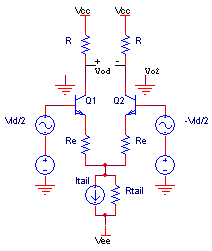
\includegraphics{schematics/differentialpair_resistorload.PNG}
\end{center}

The above differential pair is shown with a resistive load and with the optional emitter degeneration resistors $R_{E1}$ and $R_{E2}$.
The MOS version of the differential pair (the source-coupled pair) is the same but without the degeneration resistors and, of course, MOSFETs instead of $Q_{1}$ and $Q_{2}$.
The current source $I_{TAIL}$ and its output resistance $R_{TAIL}$ represent a Norton equivalent current source (usually composed of transistors, such as a current mirror), but the current source can simply consist of a resistor $R_{TAIL}$, in which $I_{TAIL} = 0$.
The bases (or gates) of the transistors are also biased to some voltage which is not necessarily equal to $GND$ (certainly not if $V_{EE} = GND$), but the bias voltages are usually equal so that $V_{B1} = V_{B2}$ (or $V_{G1} = V_{G2}$ in the MOS version).

%TODO: create figure for small signal model and minor rewrite of this paragraph
To determine the small signal differential behavior of this circuit set $I_{TAIL} = 0$ and use the bipolar hybrid-$\pi$ small signal model for the transistors (the MOS version of the circuit has a similar analysis, except with $r_{\pi} \to \infty$).
The voltage at the base of $Q_{1}$ is $\frac{v_{id}}{2}$ and the voltage at the base of $Q_{2}$ is $-\frac{v_{id}}{2}$, and the voltage at the collector of $Q_{1}$ is $\frac{v_{od}}{2}$ and the voltage at the collector of $Q_{2}$ is $-\frac{v_{od}}{2}$.
Both transistors act as voltage followers to the node that connects the two sides of the circuit (either the node that connects the emitter resistors or, if the emitter resistors are omitted, the node that connects the emitters).
Since this node is driven by equal and opposite input voltages its voltage is constant, and since its voltage is constant $R_{TAIL}$ can be shorted (which grounds the connecting node) without affecting the operation of the circuit. \autocite[226]{analysis-design-analog-ics}
Since the connecting node is grounded, the two sides of the differential pair are independent and are configured as common emitters!
The two independent sides are sometimes called \textit{differential half circuits}.
Using the above analysis of common emitters, we thus have a differential voltage gain of

\begin{equation}
\frac{v_{od}}{v_{id}} = -\frac{\beta_{F} (R \parallel r_{o})}{R_{S}' + r_{\pi}}
\end{equation}

where $r_{o}$ and $r_{\pi}$ are from the hybrid-$\pi$ small signal model and and $R_{S}'$ is defined as above. As before, we can often simplify the transfer function to

\begin{equation}
\frac{v_{od}}{v_{id}} \approx -g_m R
\label{eq:resistivediffpair_diff_gain_approx}
\end{equation}

The MOS version has a transfer function of

\begin{equation}
\frac{v_{od}}{v_{id}} = -g_{m}R
\end{equation}

since $r_{\pi} \to \infty$.

%TODO: create figure for small signal model for common-mode half circuits
A differential pair ideally has zero voltage gain for common-mode inputs.
To determine the actual small signal common-mode voltage gain use a similar approach as the differential voltage gain:
split the two sides of the circuit into two \textit{common-mode half circuits}.
To split the circuit replace $R_{TAIL}$ with two resistors in parallel with resistance $2R_{TAIL}$.
This does not modify the circuit since two identical resistors in parallel have an equivalent resistance of half the individual resistors.
The two sides are now combined only by a wire which connects the two $2R_{TAIL}$ resistors, but this wire carries no small signal current since both transistors are driven by identical input voltages ($v_{ic}$). \autocite[228]{analysis-design-analog-ics}
Consequently, the wire can be severed without affecting the circuit behavior and we have two \textit{common-mode half circuits} which are commom emitters with emitter degeneration resistances of $R_{E}+2R_{TAIL}$.
From (\ref{eq:commonemitter_transferfunction}) the common-mode voltage gain is thus

\begin{equation}
\frac{v_{oc}}{v_{ic}} = -\frac{g_{m}R}{1+g_{m}(R_{E}+2R_{TAIL})}
\label{eq:resistivediffpair_cm_gain}
\end{equation}

$R_{E}$ is usually much smaller than $2R_{TAIL}$ so the common-mode voltage gain is approximately

\begin{equation}
\frac{v_{oc}}{v_{ic}} \approx -\frac{g_{m}R}{1+2g_{m}R_{TAIL}}
\label{eq:resistivediffpair_cm_gain_approx}
\end{equation}

Using the approximate differential voltage gain (\ref{eq:resistivediffpair_diff_gain_approx}) divided by the the approximate common-mode voltage gain (\ref{eq:resistivediffpair_cm_gain_approx}) gives a good approximation of the common-mode rejection ratio CMRR, which is

\textcolor{red}{
\begin{equation}
\text{CMRR} \approx 1+2g_m R_{TAIL}
\label{eq:resistivediffpair_CMRR}
\end{equation}
}

The CMRR is strongly dependent on the value of $R_{TAIL}$ so the use of a good current source (which has an ideally infinite Norton equivalent resistance) yields a high CMRR.

The differential pair shown uses \textit{npn} transistors, but $Q_{1}$ and $Q_{2}$ can also be \textit{pnp} transistors.
If \textit{pnp} transistors are used the only difference is that $I_{TAIL}$ is sourced from $V_{CC}$ rather than sinking into $V_{EE}$.
The same is true of the MOS version of the differential pair -- PMOS transistors can be used instead of NMOS with the same change in $I_{TAIL}$.

\subsection{Differential pair with active load (GHLM, p. 278, 288)}
\begin{center}
	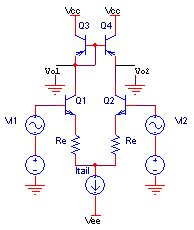
\includegraphics{schematics/differentialpair_activeload.PNG}
\end{center}
The gain of the differential pair can be increased by using an active load. $Q_{3}$ and $Q_{4}$ form a current mirror (since $Q_{3}$ is diode connected) so that $I_{TAIL}$ is split evenly and $I_{C1} = I_{C2}$. Unfortunately, the circuit is no longer symmetrical since only $Q_{3}$ is diode connected and as a result the \textsl{differential half circuit} approach used above cannot be employed.

%\subsection{Rail-to-rail differential pair (Op Amps for Everyone, p. 386)}

%\section{Wideband amplifier (my design)}